\documentclass[crop,tikz]{standalone}
\usetikzlibrary{calc}
\usetikzlibrary{arrows.meta}
\usetikzlibrary{decorations.pathreplacing}
\begin{document}
	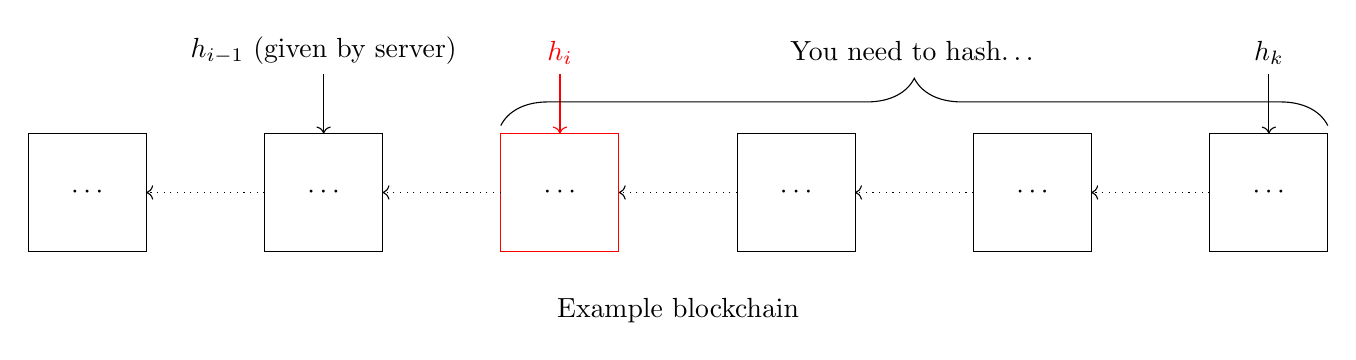
\begin{tikzpicture}[scale=1.5]
		\foreach \i in {1,2,...,6} {
			\coordinate (ledge\i) at ($2*(\i, 0) - (0.5, 0)$);
			\coordinate (redge\i) at ($2*(\i, 0) + (0.5, 0)$);
			\coordinate (ltop\i) at ($(ledge\i) + (0, 0.5)$);
			\coordinate (rbottom\i) at ($(redge\i) - (0, 0.5)$);
			\coordinate (rtop\i) at ($(redge\i) + (0, 0.5)$);
			\coordinate (ctop\i) at ($0.5*(ltop\i) + 0.5*(rtop\i)$);
			\pgfmathsetmacro\col{ifthenelse(\i==3,"red","black")}
			\path[draw=\col] (ltop\i) rectangle (rbottom\i)
				node[midway, inner sep=0pt] {$\cdots$};
		}
		\foreach \i in {2,3,...,6} {
			\pgfmathsetmacro\ii{subtract(\i,1)}
			\path[draw,dotted,->] (ledge\i) -- (redge\ii);
		}

		\path[draw,->] ($(ctop6) + (0, 0.5)$) -- (ctop6) node[at start, anchor=south] {$h_k$};
		\path[draw,red,->] ($(ctop3) + (0, 0.5)$) -- (ctop3) node[at start, anchor=south] {$h_i$};
		\path[draw,->] ($(ctop2) + (0, 0.5)$) -- (ctop2) node[at start, anchor=south] {$h_{i-1}$ (given by server)};

		\path[draw,decorate,decoration={brace,amplitude=6mm,raise=1mm}] (ltop3) -- node[above=8mm] {You need to hash\ldots} (rtop6);

		\coordinate (t) at ($0.5*($(ltop1)+(rtop6)$)$);
		\node at (t |- 0,-1) {Example blockchain};
	\end{tikzpicture}
\end{document}
